\documentclass[a4paper,10pt]{article}
\usepackage{graphicx}
\begin{document}
\thispagestyle{empty}
{\centering
Corso di Laurea in Matematica \\
LABORATORIO DIDATTICO DI MATEMATICA COMPUTAZIONALE \\
AA 2017/2018   \\
 \rule{6cm}{1pt} \\
} 
\vspace{0.3cm} \noindent
STUDENTE: Siniscalco Edoardo \\
MATRICOLA: 549781 \\

\begin{center} 
Esercizio sui Grafici \end{center}

Includiamo qui un grafico delle curve di Lissajoux ottenuto prendendo $x = \sin(2t)$ e $y = \cos(3t)$ con $t$ tra $0$ e $2\pi$

\begin{center}
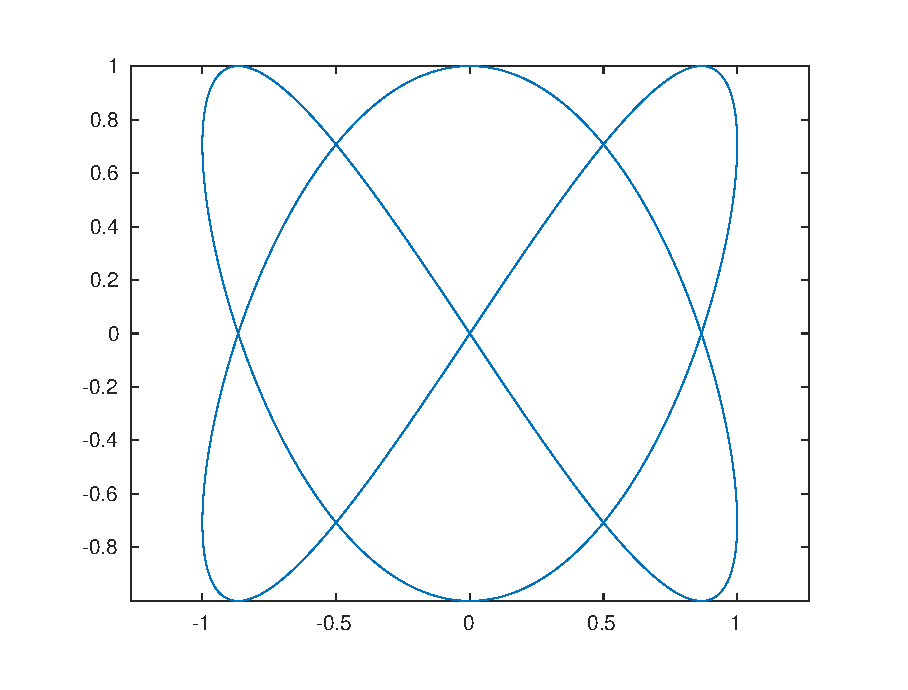
\includegraphics[scale=0.4]{fig1.eps} \end{center}

e poi un grafico tridimensionale della seguente funzione di due variabili $z = 4x^2 - 4y^2$ che mostra anche le linee di livello della funzione, rappresentata nel dominio $[-10,10] \times [-10, 10]$.

\begin{center}
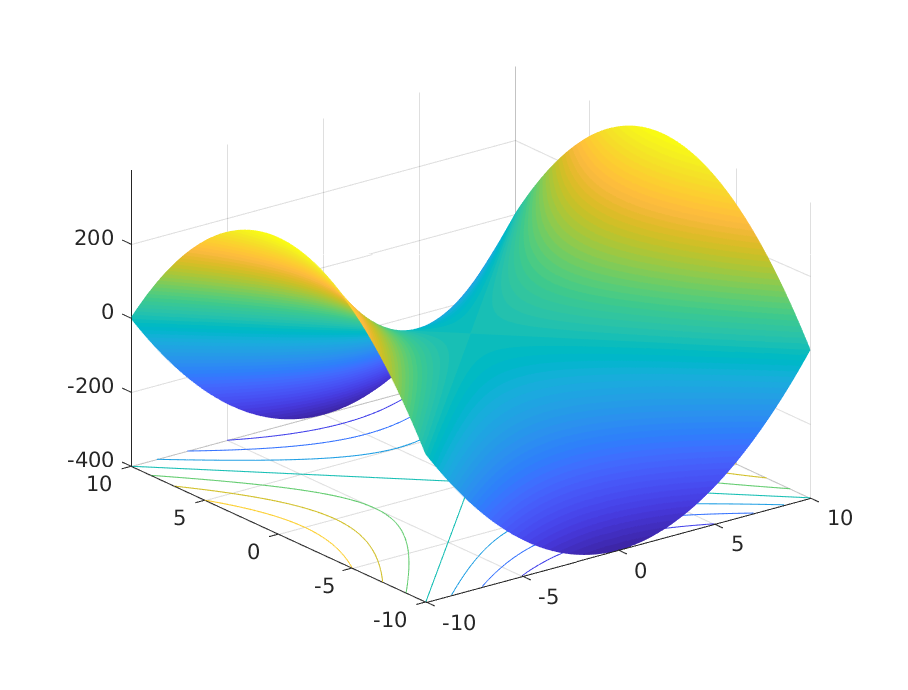
\includegraphics[scale=0.5]{fig2.eps} \end{center}

Pisa, 15 maggio 2018

\end{document}
